\section{Lezione 11}
\subsection{Esercizi: funzioni integrali}
\begin{exercise}
    \label{ex:9.1}
    Sia $f\colon\amsbb{R}\to \amsbb{R}$, $f(x) = \frac{\sin(x)}{1+x^2}$; verificare che
    \[
    F(x) = \int_0^x \frac{\sin(t)}{1+t^2}\, dt
    \]
    è ben definita su tutto $\amsbb{R}$. Inoltre,
    \begin{enumerate}[(i)]
        \item dimostrare che $F$ è pari e $F(x)\ge 0$ per ogni $x\in\amsbb{R}$;
        \item calcolare 
        \[
        \lim_{x\to 0^+} \frac{F(x)}{x^2}
        \]
    \end{enumerate}
\end{exercise}
\begin{proof}[Soluzione]
    Notiamo che $f$ è continua su tutto $\amsbb{R}$; pertanto la sua restrizione ad un intervallo del tipo $[0,x]$ per $x\ge 0$ o $[x,0]$ per $x<0$ è continua e, per il corollario \ref{cor:8.1}, integrabile su $[0,x]$ o $[x,0]$ per ogni scelta di $x\in\amsbb{R}$. Quindi $F$ è ben definita su tutto $\amsbb{R}$. Consideriamo ora i due punti:
    \begin{enumerate}[(i)]
        \item vogliamo mostrare che $F(-x) = F(x)$ per ogni $x\in\amsbb{R}$. Consideriamo per semplicità $x\ge 0$ (il caso $x<0$ è analogo) e
        \[
        F(-x) = \int_0^{-x} \frac{\sin(t)}{1+t^2}\, dt
        \]
        Notiamo che possiamo definire la funzione $\varphi\colon [0,x]\ni t\mapsto  -t\in [-x,0]$, che è differenziabile e ammette derivata continua in $[0,x]$; inoltre vale che
        \[
        F(-x) = \int_0^{-x}\frac{\sin(t)}{1+t^2}\, dt = \int_{\varphi(0)}^{\varphi(x)}\frac{\sin(t)}{1+t^2}\, dt
        \]
        Possiamo quindi usare il teorema \ref{th:8.4}: vale che
        \[
        \begin{split}
            F(-x) & = \int_{\varphi(0)}^{\varphi(x)}\frac{\sin(t)}{1+t^2}\, dt = \int_0^x \frac{\sin(-t)}{1+(-t)^2}(-1)\, dt = -\int_0^x \frac{-\sin(t)}{1+t^2}\, dt = \int_0^x \frac{\sin(t)}{1+t^2}\, dt = \\
            & = F(x)
        \end{split}
        \]
        ove abbiamo usato il fatto che $\sin(\cdot)\colon\amsbb{R}\to\amsbb{R}$ è dispari.\\
        Alla luce di questo, per verificare che $F(x)\ge 0$ per ogni $x\in\amsbb{R}$, possiamo restringerci a $\amsbb{R}^+$. Purtroppo, $F(x)$ non ammette un'espressione in termini di funzioni elementari; per capire se $F(x)\ge 0$ per ogni $x\in\amsbb{R}^+$ è quindi necessario agire in altro modo. Possiamo, per esempio, studiarne il comportamento, studiando la sua derivata prima. Innanzitutto, notiamo che $f$ è continua su tutto $\amsbb{R}^+$, e di conseguenza per il teorema \ref{th:8.2} $F$ è differenziabile in tutto $\amsbb{R}^+$; vale inoltre che
        \[
        F'(x) = \frac{\sin(x)}{1+x^2} \ \text{per ogni} \ x\in\amsbb{R}^+
        \]
        Notiamo che, dato $k\in\amsbb{N}$,
        \[
        F'(x)\ge 0 \ \text{se} \ x\in[2k\pi, 2k\pi + \pi] \ \text{e} \ F'(x)\le 0 \ \text{se} \ x\in(2k\pi+\pi, 2(k+1)\pi]
        \]
        ossia
        \begin{center}
            \begin{tikzpicture}
                \tikzset{h style/.style = {fill=black!30}}
                \tkzTabInit[lgt=3,espcl=2.5, deltacl=1.5]
                { /.8, $F'(x) = f(x)$ /.8, $F(x)$ /.8}
                {$2k\pi $, $2k\pi + \pi $, $2(k+1)\pi$, $2(k+1)\pi + \pi$ } % four main references
                \tkzTabLine{ z, +,z,-, z, +, z } % seven denotations
                \tkzTabVar{ -/ , +/, -/, +/ }%
            \end{tikzpicture}
        \end{center}
        Quindi $F$ cresce da $2k\pi$ a $2k\pi + \pi$, decresce fino a $2(k+1)\pi$ e poi ripete il ciclo. Di conseguenza, per dimostrare che $F$ è positiva è sufficiente mostrare che $F(2k\pi)\ge 0$ per ogni $k\in\amsbb{N}$, poiché dallo studio del segno di $F'$ possiamo concludere che $F(x)\ge F(2k\pi)$ per ogni $x\in[2k\pi -\pi , 2k\pi +\pi]$. Poiché al variare di $k\in\amsbb{N}$ questi intervalli costituiscono una partizione di $\amsbb{R}^+$ avremmo allora che $F(x)\ge 0$ per ogni $x\in\amsbb{R}^+$.\\
        Calcoliamo quindi $F(2k\pi)$ al variare di $k\in\amsbb{N}$: chiaramente per $k=0$ abbiamo
        \[
        F(0) =  \int_0^0 \frac{\sin(t)}{1+t^2}\, dt = 0
        \]
        Per un $k$ generico vale invece che
        \[
        F(2k\pi) = \int_0^{2k\pi}\frac{\sin(t)}{1+t^2}\, dt
        \]
        che possiamo scrivere come
        \[
        \sum_{i=0}^{k-1}\bigg(\underbrace{\int_{2i\pi}^{2i\pi +\pi} \frac{\sin(t)}{1+t^2}\, dt}_{\stepcounter{equation}\mbox{(\theequation)}} + \underbrace{\int_{2i\pi + \pi }^{2(i+1)\pi} \frac{\sin(t)}{1+t^2}\, dt}_{\stepcounter{equation}\mbox{(\theequation)}}\bigg)
        \]
        \addtocounter{equation}{-2}\refstepcounter{equation}\label{eq:9.1}
        \addtocounter{equation}{0}\refstepcounter{equation}\label{eq:9.2}
        Notiamo che se consideriamo la funzione $\varphi\colon [2i\pi, 2i\pi + \pi]\ni t \mapsto t+\pi$ abbiamo che l'integrale (\ref{eq:9.2}) può essere scritto come
        \[
        \begin{split}
            \int_{2i\pi +\pi}^{2(i+1)\pi} \frac{\sin(t)}{1+t^2}\, dt &= \int_{\varphi(2i\pi)}^{\varphi(2i\pi +\pi)} \frac{\sin(t)}{1+t^2}\, dt \overset{\text{Teorema \ref{th:8.4}}}{=} \int_{2i\pi}^{2i\pi +\pi} \frac{\sin(t+\pi)}{1+(t+\pi)^2}\, dt = \\
            & = -\int_{2i\pi}^{2i\pi +\pi} \frac{\sin(t)}{1+(t+\pi)^2}\, dt
        \end{split}
        \]
        Notiamo che 
        \[
        1+t^2 \le 1+(t+\pi)^2 \implies \frac{1}{1+t^2}\ge \frac{1}{1+(t+\pi)^2} \ \text{per ogni} \ t\in[2i\pi, 2i\pi+\pi]
        \]
        e, poiché $\sin(t)\ge 0$ in $[2i\pi, 2i\pi+\pi]$ vale che 
        \[
        \frac{\sin(t)}{1+t^2}\ge \frac{\sin(t)}{1+(t+\pi)^2} \iff \frac{\sin(t)}{1+t^2}- \frac{\sin(t)}{1+(t+\pi)^2}\ge 0 \ \text{per ogni} \ t\in[2i\pi, 2i\pi + \pi]
        \]
        Di conseguenza abbiamo che
        \[
        \begin{split}
            \int_0^{2k\pi} \frac{\sin(t)}{1+t^2}\, dt & = \sum_{i=0}^{k-1} \left({\int_{2i\pi}^{2i\pi +\pi} \frac{\sin(t)}{1+t^2}\, dt} + {\int_{2i\pi + \pi }^{2(i+1)\pi} \frac{\sin(t)}{1+t^2}\, dt}\right) = \\
            & = \sum_{i=0}^{k-1} \bigg(\int_{2i\pi}^{2i\pi +\pi} \underbrace{\frac{\sin(t)}{1+t^2} - \frac{\sin(t)}{1+(t+\pi)^2}}_{\ge 0}\, dt\bigg)\ge 0
        \end{split}
        \]
        Abbiamo quindi provato che $F(2k\pi)\ge 0$ per ogni $k\in\amsbb{N}$, e di conseguenza $F(x)\ge 0$ per ogni $x\in\amsbb{R}$.
        \item Vogliamo calcolare 
        \[
        \lim_{x\to 0^+} \frac{F(x)}{x^2}
        \]
        Notiamo che il limite è una forma indeterminata del tipo $\left[\frac{0}{0}\right]$; possiamo quindi provare ad applicare il teorema di de l'H{\^o}pital \ref{th:6.4}. Notiamo che $F(x)$ e $x^2$ sono entrambe differenziabili in $(0,+\infty)$, con
        \[
        F'(x) = f(x) = \frac{\sin(x)}{1+x^2} \qquad \frac{d}{dx}(x^2) = 2x\ne 0 \ \text{in} \ (0,+\infty)
        \]
        Inoltre,
        \[
        \lim_{x\to 0^+} \frac{F'(x)}{2x} = \lim_{x\to 0^+} \frac{\sin(x)}{2x}\frac{1}{1+x^2} = \frac{1}{2}
        \]
        Di conseguenza per il teorema di de l'H{\^o}pital abbiamo che
        \[
        \lim_{x\to 0^+} \frac{F(x)}{x^2} = \frac{1}{2}
        \]
    \end{enumerate}
\end{proof}
\begin{exercise}
    \label{ex:9.2}
    Data $g\colon \amsbb{R}\to \amsbb{R}$,
    \[
    g(x) = \int_0^{x^2}\cos(2t)\, dt
    \]
    determinarne, se esistono, i punti critici e calcolare 
    \[
    \lim_{x\to 0^+} \frac{g(x)-x^2}{x^6}
    \]
\end{exercise}
\begin{proof}[Soluzione]
    Notiamo che $g$ può essere scritta come la composizione di due funzioni,
    \[
    g = F \circ h, \quad F(x) = \int_0^x \cos(2t)\, dt \quad h(x) = x^2
    \]
    Dato che $\amsbb{R}\ni t \mapsto \cos(2t)$ è continua su tutto $\amsbb{R}$, ragionando come nell'esercizio \ref{ex:9.1} abbiamo che $F(x)$ è differenziabile su tutto $\amsbb{R}$, con $F'(x) = \cos(2x)$. Quindi $g$, essendo la composizione di due funzioni differenziabili su tutto $\amsbb{R}$, è differenziabile su tutto $\amsbb{R}$, e usando la (\ref{eq:6.4}) vale che che
    \[
    g'(x) = (F \circ h)'(x) = F'(h(x))h'(x) = 2x\cos(2x^2)
    \]
    I punti stazionari di $g$ saranno dati dagli zeri di $g'$; questo accade se $x=0$ o se $\cos(2x^2)=0$, ossia se
    \[
    x=0 \lor 2x^2 = \frac{\pi}{2}+k\pi \iff x=\pm\sqrt{\frac{\pi}{4}+k\frac{\pi}{2}}, \ k\in\amsbb{N}
    \]
    Vogliamo capire se i punti critici in questione sono massimi o minimi locali; per fare questo, studiamo il segno della derivata: in prossimità di $x=0$ vale che
    \begin{center}
        \begin{tikzpicture}
            \tikzset{h style/.style = {fill=black!30}}
            \tkzTabInit[lgt=2,espcl=2.5, deltacl=1.5]
            { /.8, $g'(x)$ /.8, $g(x)$ /.8}
            {$-\sqrt{\frac{\pi}{4}}$, $0$, $\sqrt{\frac{\pi}{4}}$ } % four main references
            \tkzTabLine{ z, -, z,+ , z } % seven denotations
            \tkzTabVar{ +/ , -/, +/}%
        \end{tikzpicture}
    \end{center}
    e di conseguenza $x=0$ è un punto di minimo locale per $g$. Per quanto riguarda invece i punti $x= \sqrt{\frac{\pi}{4}+k\frac{\pi}{2}}$ abbiamo che, per $k$ pari,
    \begin{center}
        \begin{tikzpicture}
            \tikzset{h style/.style = {fill=black!30}}
            \tkzTabInit[lgt=2,espcl=3.3, deltacl=1.5]
            { /.8, $g'(x)$ /.8, $g(x)$ /.8}
            {$\sqrt{\frac{\pi}{4}+k\frac{\pi}{2}}$, $\sqrt{\frac{\pi}{4}+(k+1)\frac{\pi}{2}}$, $\sqrt{\frac{\pi}{4}+(k+2)\frac{\pi}{2}}$ } % four main references
            \tkzTabLine{ z, -, z,+ , z } % seven denotations
            \tkzTabVar{ +/ , -/, +/}%
        \end{tikzpicture}
    \end{center}
    ossia 
    \[
    x= \sqrt{\frac{\pi}{4}+2n\frac{\pi}{2}} \ \text{massimi locali e} \ x= \sqrt{\frac{\pi}{4}+(2n+1)\frac{\pi}{2}} \ \text{minimi locali},\ n\in\amsbb{N}
    \]
    Per quanto riguarda invece $x=-\sqrt{\frac{\pi}{4}+k\frac{\pi}{2}}$, abbiamo che, supponendo sempre $k$ pari,
    \begin{center}
        \begin{tikzpicture}
            \tikzset{h style/.style = {fill=black!30}}
            \tkzTabInit[lgt=2,espcl=3.3, deltacl=1.5]
            { /.8, $g'(x)$ /.8, $g(x)$ /.8}
            {$-\sqrt{\frac{\pi}{4}+(k+2)\frac{\pi}{2}}$,  $-\sqrt{\frac{\pi}{4}+(k+1)\frac{\pi}{2}}$, $-\sqrt{\frac{\pi}{4}+k\frac{\pi}{2}}$ } % four main references
            \tkzTabLine{ z, -, z,+ , z } % seven denotations
            \tkzTabVar{ +/ , -/, +/}%
        \end{tikzpicture}
    \end{center}
    ossia 
    \[
    x= -\sqrt{\frac{\pi}{4}+2n\frac{\pi}{2}} \ \text{massimi locali e} \ x= -\sqrt{\frac{\pi}{4}+(2n+1)\frac{\pi}{2}} \ \text{minimi locali},\ n\in\amsbb{N}
    \]
    Calcoliamo ora 
    \[
    \lim_{x\to 0^+} \frac{g(x)-x^2}{x^6}
    \]
    Come nel caso dell'esercizio precedente, il limite è una forma indeterminata del tipo $\left[\frac{0}{0}\right]$, e di conseguenza possiamo provare ad applicare il teorema di de l'H{\^o}pital \ref{th:6.4}: vale che $g(x)-x^2$ e $x^6$ sono differenziabili su tutto $(0,+\infty)$, con $g'(x)-2x = 2x(\cos(2x^2)-1)$ e $(x^6)' = 6x^5\ne 0$ per $x\in(0,+\infty)$, e inoltre
    \[
    \begin{split}
        \lim_{x\to 0^+} \frac{g'(x)-2x}{6x^5} & = \lim_{x\to 0^+} \frac{2x(\cos(2x^2)-1)}{6x^5} \overset{(\ref{eq:5.12})}{=} \lim_{x\to 0^+}\frac{2x(1-2x^4+o(x^4)-1}{6x^5} = \\
        & = \lim_{x\to 0^+} \frac{-4x^5+o(x^5)}{6x^5} = -\frac{2}{3}
    \end{split}
    \]
    Di conseguenza possiamo applicare il teorema di de l'H{\^o}pital e concludere che
    \[
    \lim_{x\to 0^+} \frac{g(x)-x^2}{x^6} = -\frac{2}{3}
    \]
\end{proof}
\begin{exercise}
    \label{ex:9.3}
    Data la funzione $F\colon\amsbb{R}^+\to \amsbb{R}$,
    \[
    F(x) = \int_{x^2+x}^{2x^2}\frac{1}{1+t\log(t)}\, dt
    \]
    calcolare i primi due termini dello sviluppo di Taylor di $F$ centrato in $x_0=1$.
\end{exercise}
\begin{proof}[Soluzione]
    Notiamo che la funzione $F$ è ben definita su tutto $\mathbb{R}^+$: infatti, la funzione integranda $\mathbb{R}^+\ni t \mapsto \frac{1}{1+t\log(t)}$ è continua e ben definita su tutto $\mathbb{R}^+$. Per mostrarlo, possiamo considerare il seguente fatto: notiamo che $\mathbb{R}^+\ni t\mapsto 1+t\log(t)$ è sempre positiva, infatti abbiamo che
    \begin{enumerate}[(i)]
        \item $\lim_{t\to 0^+} 1+t\log(t)=1$;
        \item $1+t\log(t)$ è derivabile su tutto $\mathbb{R}^+$, e la sua derivata prima è $1+\log(t)$. Questa si annulla solamente in $\frac{1}{e}$, ed è negativa in $\left(0, \frac{1}{e}\right)$ e positiva in $\left(\frac{1}{e}, +\infty\right)$; di conseguenza $\frac{1}{e}$ è un punto di minimo globale della funzione, e $1+\frac{1}{e}\log\left(\frac{1}{e}\right)=\frac{e-1}{e}>0$.
    \end{enumerate}
    Di conseguenza $(1+t\log(t))^{-1}$ è ben definita su tutto $\mathbb{R}^+$ ed è continua, essendo composizione di funzioni continue.\\
    Dall'esercizio \ref{ex:9.2} sappiamo calcolare le derivate di oggetti del tipo
    \[
    \int_{a}^{f(x)} g(t)\, dt
    \]
    Dobbiamo pertanto ricondurci ad una forma simile. Sappiamo che la funzione integranda è definita in $1$; possiamo pertanto scrivere
    \[
    \begin{split}
        F(x) & = \int_{x^2+x}^{2x^2}\frac{1}{1+t\log(t)}\, dt = \int_{1}^{2x^2}\frac{1}{1+t\log(t)}\, dt + \int_{x^2+x}^1\frac{1}{1+t\log(t)}\, dt = \\
        & = \int_1^{2x^2} \frac{1}{1+t\log(t)}\, dt -\int_1^{x^2+x}\frac{1}{1+t\log(t)}\, dt
    \end{split}
    \]
    A questo punto osserviamo che la funzione integranda è continua in $(0,+\infty)$, e di conseguenza, grazie al teorema \ref{th:8.2}, $F$ è differenziabile in $(0,+\infty)$, essendo somma e composizione di funzioni differenziabili. Vale in particolare che
    \[
    F'(x) \overset{(\ref{eq:6.4})}{=} \frac{4x}{1+2x^2\log(2x^2)} -\frac{2x+1}{1+(x^2+x)\log(x^2+x)}
    \]
    Ricordiamo che il polinomio di Taylor di una funzione ha la forma (\ref{eq:6.7}); di conseguenza è necessario calcolare $F(1)$, $F'(1)$ e $F''(1)$. Chiaramente vale che
    \[
    F(1) = \int_2^2 \frac{1}{1+t\log(t)}\, dt = 0
    \]
    mentre
    \[
    F'(1) = \frac{4}{1+2\log(2)}-\frac{3}{1+2\log(2)} = \frac{1}{1+2\log(2)}
    \]
    Dobbiamo ora calcolare $F''(x)$:
    \[
    \begin{split}
        F''(x) & = \frac{4}{1+2x^2\log(2x^2)}-\frac{(4x)^2}{(1+2x^2\log(2x^2))^2}\left(\log(2x^2)+1\right)- \\
        & - \frac{2}{1+(x^2+x)\log(x^2+x)}+\frac{(2x+1)^2}{(1+(x^2+x)\log(x^2+x))^2}\left(\log(x^2+x)+1\right)
    \end{split}
    \]
    Se valutiamo l'espressione in $x_0=1$ otteniamo
    \[
    \begin{split}
        F''(1) & = \frac{4}{1+2\log(2)}-\frac{16}{(1+2\log(2))^2}(\log(2)+1)-\\
        & - \frac{2}{1+2\log(2)}+\frac{9}{(1+2\log(2))^2}(\log(2)+1) = \\
        & = \frac{2}{1+2\log(2)}-\frac{7}{(1+2\log(2))^2}(1+\log(2)) =\\
        & = \frac{-5-3\log(2)}{(1+2\log(2))^2}
    \end{split}
    \]
    Possiamo quindi scrivere
    \[
    F(x) = 0 + \frac{1}{1+2\log(2)}(x-1)-\frac{5+3\log(2)}{(1+2\log(2))^2}(x-1)^2 +o((x-1)^2)
    \]
\end{proof}
\begin{exercise}
    \label{ex:9.4}
    Data la successione $(a_n)_n$, 
    \[
    a_n = \int_0^1 n e^{-nx}\, dx
    \]
    determinarne, se esiste, il limite per $n\to\infty$
\end{exercise}
\begin{proof}[Soluzione]
    Notiamo che se fissiamo $x_0\in(0,1]$ la successione $b_n = ne^{-nx_0} $ tende a 0 per $n\to \infty$, mentre se consideriamo $x_0=0$ vale che $b_n = n $ diverge a $+\infty$. Se immaginiamo di poter fare lo scambio
    \[
    \lim_{n\to\infty}\int_0^1 ne^{-nx}\, dx = \int_0^1 \lim_{n\to \infty} ne^{-nx}\, dx
    \]
    possiamo pensare, alla luce del corollario \ref{cor:8.2}, che 
    \[
    \int_0^1 \lim_{n\to \infty} ne^{-nx}\, dx = 0
    \]
    Tuttavia, se effettuiamo esplicitamente il calcolo vale che
    \[
    a_n = \int_0^1 ne^{-nx}\, dx = -\int_0^1 e^{-nx}(-n)\, dx \overset{\text{Teorema \ref{th:8.4}}}{=} -\int_0^{-n} e^{y}\, dy = 1-e^{-n}  
    \]
    e di conseguenza
    \[
    \lim_{n\to\infty} a_n = \lim_{n\to\infty}1-e^{-n} = 1
    \]
    Abbiamo quindi verificato che, almeno in questo caso, 
    \[
    \lim_{n\to\infty}\int_0^1 ne^{-nx}\, dx \ne \int_0^1 \lim_{n\to \infty} ne^{-nx}\, dx
    \]
\end{proof}
\begin{exercise}
    \label{ex:9.5}
    Data la successione $(a_n)_n$,
    \[
    a_n = \int_0^{\frac{\pi}{4}} \tan^n(x)\, dx
    \]
    determinarne, se esiste, il limite per $n\to\infty$.
\end{exercise}
\begin{proof}[Soluzione]
    Anche in questo caso la funzione integranda ha un comportamento simile alla funzione integranda dell'esercizio \ref{ex:9.5}: infatti per $x_0\in\left(0, \frac{\pi}{4}\right)$ vale che $b_n = \tan^n(x_0)\to 0$ per $n\to\infty$, mentre per $x_0=\frac{\pi}{4}$ vale che $b_n = 1$ per ogni $n\in\amsbb{N}$. Quindi, ragionando per analogia con il caso dell'esercizio \ref{ex:9.5}, a priori non possiamo scambiare l'operazione di limite e l'integrazione. Calcoliamo quindi
    \[
    \int_0^{\frac{\pi}{4}}\tan^n(x)\, dx
    \]
    Notiamo innanzitutto che, poiché $\tan(x)\le 1$ per ogni $x\in\left[0, \frac{\pi}{4}\right]$, vale che, per ogni $n\in\amsbb{N}$
    \[
    \tan^{n+1}(x)\le \tan^{n}(x) \ \text{per ogni} \ x\in\left[0, \frac{\pi}{4}\right]
    \]
    Quindi per ogni $n\in\amsbb{N}$
    \[
    \int_0^{\frac{\pi}{4}}\tan^n(x)\, dx \ge \int_0^{\frac{\pi}{4}}\tan^{n+1}(x)\, dx
    \]
    ossia $a_n \ge a_{n+1}$, e quindi la successione è monotona decrescente. Vale inoltre che per ogni $n\in\amsbb{N}$,  $\tan^n(x)\ge 0$; di conseguenza
    \[
    \int_0^{\frac{\pi}{4}}\tan^n(x)\, dx \ge 0 \ \text{per ogni} \ n\in\amsbb{N}
    \]
    ossia $a_n\ge 0$. Quindi per il teorema \ref{th:4.7} $a_n\to a$ per $n\to \infty$. Per determinare $a$, calcoliamo esplicitamente l'integrale: chiaramente per $n=0$ vale che
    \[
    a_0 = \int_0^{\frac{\pi}{4}}\tan^0(x)\, dx = \int_0^{\frac{\pi}{4}}1\, dx =\frac{\pi}{4} 
    \]
    mentre per $n=1$ abbiamo
    \[
    \begin{split}
        a_1 & = \int_0^{\frac{\pi}{4}}\tan(x)\, dx =\int_0^{\frac{\pi}{4}}\frac{\sin(x)}{\cos(x)}\, dx  = -\int_0^{\frac{\pi}{4}} \frac{1}{\cos(x)}\frac{d}{dx}(\cos(x))\, dx \overset{\text{Teorema \ref{th:8.4}}}{=}\\
        & =  -\int_1^{\frac{\sqrt{2}}{2}} \frac{1}{t}\, dt = -\log{\abs{t}}\bigg|_1^{\frac{\sqrt{2}}{2}} = -\log\left(\frac{1}{\sqrt{2}}\right) = \frac{1}{2}\log(2)
    \end{split}
    \]
    Supponiamo ora che $n\ge 2$: possiamo scrivere
    \[
    \begin{split}
        a_n  & = \int_0^{\frac{\pi}{4}}\tan^n(x)\, dx = \int_0^{\frac{\pi}{4}} \tan^{n-2}(x)\tan^2(x)\, dx = \int_0^{\frac{\pi}{4}} \tan^{n-2}(x) \frac{\sin^2(x)}{\cos^2(x)}\, dx =\\
        & = \int_0^{\frac{\pi}{4}} \tan^{n-2}(x) \frac{1-\cos^2(x)}{\cos^2(x)}\, dx = \int_0^{\frac{\pi}{4}} \tan^{n-2}(x) \frac{1}{\cos^2(x)}\, dx - \int_0^{\frac{\pi}{4}} \tan^{n-2}(x)\, dx = \\
        & = \int_0^{\frac{\pi}{4}}\tan^{n-2}(x) \frac{d}{dx}(\tan(x))\, dx - a_{n-2} = \overset{\text{Teorema \ref{th:8.4}}}{=} \int_0^1 y^{n-2}\, dy - a_{n-2} = \\
        & = \frac{1}{n-1} y^{n-1}\bigg|_0^1 - a_{n-2} = \frac{1}{n-1}-a_{n-2}
    \end{split}
    \]
    Abbiamo quindi che
    \[
    a = \lim_{n\to \infty} a_n = \lim_{n\to\infty}\left( \frac{1}{n-1} - a_{n-2}\right) = -\lim_{n\to\infty}a_{n-2} = -a
    \]
    ossia il limite della successione soddisfa $a=-a$; l'unico numero reale che verifica questa uguaglianza è $0$, quindi $a=0$ e
    \[
    \lim_{n\to\infty} \int_0^{\frac{\pi}{4}} \tan^n(x)\, dx = 0
    \]
    In questo caso vale che
    \[
    \lim_{n\to\infty} \int_0^{\frac{\pi}{4}} \tan^n(x)\, dx = \int_0^{\frac{\pi}{4}}\lim_{n\to\infty} \tan^n(x)\, dx
    \]
\end{proof}
\begin{exercise}
    \label{ex:9.6}
    Data la funzione $f\colon\amsbb{R}^+\to \amsbb{R}$,
    \[
    f(x) = \int_0^1 \frac{t^4}{(t+x^2)^3}\, dt
    \]
    determinare
    \[
    \lim_{x\to 0^+} f(x)
    \]
\end{exercise}
\begin{proof}[Soluzione]
    In generale, abbiamo visto negli esercizi \ref{ex:9.4} e \ref{ex:9.5} che lo scambio di limite ed integrazione non porta al giusto risultato. Per risolvere l'esercizio possiamo procedere in due modi:
    \begin{enumerate}[(i)]
        \item Calcoliamo esplicitamente l'integrale:
        \[
        \begin{split}
            &\int_0^1 \frac{t^4}{(t+x^2)^3}\, dt = \int_0^1 \frac{t^4}{x^6\left(1+\frac{t}{x^2}\right)^3}\, dt = x^4\int_0^1\frac{t^4}{x^8}\frac{1}{\left(1+\frac{t}{x^2}\right)^3} \frac{1}{x^2}\, dt \overset{\text{Teorema \ref{th:8.4}}}{=} \\
            & = x^4\int_0^{\frac{1}{x^2}} \frac{u^4}{(1+u)^3}\, du \overset{\text{Teorema \ref{th:8.5}}}{=} -\frac{1}{2(x^2+1)^2} +\frac{x^4}{2}\int_0^{\frac{1}{x^2}}\frac{4u^3}{(1+u)^2}\, du \overset{\text{Teorema \ref{th:8.5}}}{=}\\
            & = -\frac{1}{2(x^2+1)^2}-\frac{2}{(x^2+1)}+6x^4\int_0^{\frac{1}{x^2}}\frac{u^2}{u+1}\, du = \\
            & = -\frac{1}{2(x^2+1)^2}-\frac{2}{(x^2+1)}+6\int_0^{\frac{1}{x^2}}\frac{u^2-1+1}{u+1}\, du = \\
            & = -\frac{1}{2(x^2+1)^2}-\frac{2}{(x^2+1)}+6x^4\int_0^{\frac{1}{x^2}} u-1\, du + 6x^4 \int_0^{\frac{1}{x^2}} \frac{1}{u+1}\, du  = \\
            & = -\frac{1}{2(x^2+1)^2}-\frac{2}{(x^2+1)} + \frac{6x^4}{2x^4} - \frac{6x^4}{x^2} + 6x^4\log\left(1+\frac{1}{x^2}\right) = \\
            & = 3 -\frac{1}{2(x^2+1)^2}-\frac{2}{(x^2+1)} - 6{x^2} + 6x^4\log\left(1+\frac{1}{x^2}\right)
        \end{split}
        \]
        Se effettuiamo il limite esplicitamente otteniamo
        \[
        \begin{split}
            \lim_{x\to 0^+} \int_0^1 \frac{t^4}{(t+x^2)^3}\, dt &= \lim_{x\to 0^+} 3 -\frac{1}{2(x^2+1)^2}-\frac{2}{(x^2+1)} - 6{x^2} + 6x^4\log\left(1+\frac{1}{x^2}\right) = \\
            & = 3-2-\frac{1}{2} = \frac{1}{2}
        \end{split}
        \]
        \item Possiamo effettuare la seguente manipolazione, restringendo il dominio della funzione integranda a $(0,1]$ (che non comporta problemi all'integrazione, cfr. corollario \ref{cor:8.2}):
        \[
        f(x) = \int_0^1 \frac{t^4}{(t+x^2)^3}\, dt = \int_0^1 \frac{t^4}{t^3\left(1+\frac{x^2}{t}\right)^3}\, dt = \int_0^1 \frac{t}{\left(1+\frac{x^2}{t}\right)^3}
        \]
        A questo punto, possiamo considerare lo sviluppo di Taylor di $\left(1+\frac{x^2}{t}\right)^{-3}$ in un intorno di 0:
        \[
        \left(1+\frac{x^2}{t}\right)^{-3} = 1 -3\frac{x^2}{t} + o(x^2)
        \]
        e sostituire questa espressione nell'integrale, ottenendo
        \[
        \begin{split}
            f(x) & = \int_0^1 t\left(1+\frac{x^2}{t}\right)^{-3} = \int_0^1 t\left(1-3\frac{x^2}{t}+o(x^2)\right)\, dt = \int_0^1 t - 3x^2 + to(x^2)\, dt = \\
            & = \left(\frac{t^2}{2}-3x^2t+o(x^2)\frac{t^2}{2}\right)\bigg|_0^1 = \frac{1}{2}-3x^2 +o(x^2)
        \end{split}
        \]
        e quindi
        \[
        \lim_{x\to 0^+} \frac{1}{2}-3x^2 +o(x^2) = \frac{1}{2}
        \]
    \end{enumerate} 
\end{proof}
\begin{remark}
    Come abbiamo visto in precedenza, in generale lo scambio dell'operazione di limite con l'operazione di integrazione non è consentito. Quindi ci chiediamo se la procedura risolutiva che abbiamo adottato nel punto (ii) sia o meno legittima.\\
    In generale, i teoremi che regolano questa procedura sono tre: il teorema della convergenza monotona, il teorema della convergenza uniforme e il teorema della convergenza dominata\footnote{Ne esistono diverse versioni: quella applicabile all'integrazione di Riemann è dovuta ad Arzelà, mentre la versione per l'integrazione di Lebesgue è detta convergenza dominata di Lebesgue. I due teoremi differiscono per un'ipotesi fondamentale: il primo assume che la successione di funzioni converga puntualmente ad una funzione integrabile secondo Riemann, mentre per il secondo è sufficiente che la successione converga puntualmente.}. Nel caso in esame, le richieste del teorema della convergenza dominata di Arzelà \cite{Arzelà_1885} sono soddisfatte: infatti,
    \begin{enumerate}[(i)]
        \item data una qualsiasi successione $(x_n)_n\subseteq \mathbb{R}^+$ che converge a $0$, abbiamo che la successione di funzioni $[0,1]\ni t \mapsto i_n(t) = t^4(t+x_n^2)^{-3}$ converge puntualmente a
        \[
        \lim_{n\to \infty} i_n(t) =  \lim_{n\to\infty} t^4(t+x_n^2)^{-3} = t
        \]
        Chiaramente $t\in\mathscr{R}([0,1])$. 
        \item data una qualsiasi successione $(x_n)_n$ con $x_n \to 0^+$, abbiamo che
        \[
        \abs{i_n(t)} = \abs{t^4(t+x_n^2)^{-3}} \le \abs{t} \le 1
        \]
        ossia $\abs{i_n(t)}\le 1$ per ogni $t\in[0,1]$, per ogni $n\in\mathbb{N}$.
    \end{enumerate}
         Quindi in questo caso la procedura di scambio è consentita, e abbiamo
        \[
        \lim_{x\to 0^+} \int_0^1 \frac{t^4}{(t+x^2)^3}\, dt = \int_0^1 \lim_{x\to 0^+} \frac{t^4}{(t+x^2)^3}\, dt
        \]
        L'espansione di Taylor della funzione integranda è quindi giustificata.
        \emph{Ai fini dell'esame, se vi troverete davanti un caso simile all'esercizio \ref{ex:9.6}, le ipotesi del teorema della convergenza dominata di Arzelà saranno soddisfatte.}\\
         
\end{remark}
\newpage